\documentclass{standalone}
\usepackage{pgfplots}
\pgfplotsset{width=7cm,compat=1.17}
\begin{document}
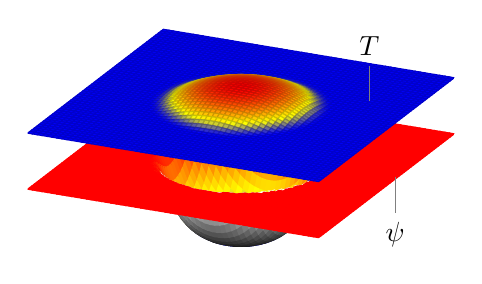
\begin{tikzpicture}
\begin{axis}[
% title=Temperature bump and corresponding gravity potential,  
hide axis,
zmax=1,
point meta rel=per plot,
mesh/interior colormap name=hot,
colormap/blackwhite,
]


%% Gravity
\addplot3 [
surf,
domain=-1.7:1.7,
samples=60,
shader=flat,
] {
  -ln(ifthenelse(abs(x^2 + y^2)<1,exp(-1/(1-x^2 - y^2)), 0)/0.1 + 1 ) - 1
};
%% Temperature
\addplot3 [
surf,
domain=-1.7:1.7,
samples=60,
shader=faceted,
] {
  ifthenelse(abs(x^2 + y^2)<1,exp(-1/(1-x^2 - y^2)), 0) + 0.1
};

\node [coordinate,pin=above:{$T$}] at (axis cs:1.5,0,0.6) {};
\node [coordinate,pin=below:{$\psi$}] at (axis cs:1.8,0,-0.8) {};
\end{axis}
\end{tikzpicture}
\end{document}